\documentclass[10pt]{article} % For LaTeX2e

% This template and styling file have been adapted from the ML Reproducibility Challenge 2020 and TMLR templates, to ease the submission.

% Switch to \usepackage[instructions]{atml} to see the general instructions again.
\usepackage{atml}

\input{math_commands.tex}

\usepackage{hyperref}
\usepackage{url}
\usepackage{booktabs}
\usepackage{xcolor}
\usepackage{graphicx}
\usepackage{amsmath}

% Every unfinished spot is marked with \todo{...}; grep for "todo" before submitting.
\newcommand{\todo}[1]{\textcolor{red}{[TODO: #1]}}

\title{[Re] PINNsFormer: A Transformer-Based Framework For Physics-Informed Neural Networks}

\author{%
  \name Diell Kryeziu \email diell.kryeziu@usi.ch
}

\def\groupid{---}
\def\projectid{PINNsFormer}


\begin{document}

\maketitle

\begin{abstract}
We study the reproducibility of PINNsFormer \citep{zhao2024pinnsformer}, a Transformer-based architecture for physics-informed neural networks (PINNs) that expands each collocation point into a short pseudo-sequence in time, processes it with a small encoder--decoder, and uses a learnable $\omega_1\sin x+\omega_2\cos x$ ``Wavelet'' activation. Its central claim is that this escapes the known failure modes of PINNs on the convection and 1D-reaction equations. Using the authors' code, wrapped in a single runner, we re-run the main comparison against three MLP baselines and add experiments the paper lacks: multiple seeds, a PINN with the Wavelet activation, PINNsFormer with sequence length one, matched training meshes, a doubled iteration budget, and the activation ablation. The 1D-reaction result reproduces (rMAE $0.016\pm0.003$ over three seeds; published $0.015$). The convection result does not: the authors' configuration fails on every run, while their pretrained checkpoint and, unexpectedly, PINNsFormer with sequence length one both reach the published error. On 1D-wave the plain PINN beats PINNsFormer. Seeds change the outcome for baselines and PINNsFormer alike, a plain sine activation matches Wavelet, and a larger mesh does not help. We conclude that the empirical claim is only partly reproducible and that the paper's explanation in terms of temporal dependencies is not supported by the convection experiment.
\end{abstract}

%%%%

\section{Introduction}
Physics-informed neural networks \citep{raissi2019pinns} approximate the solution $u(\vx,t)$ of a PDE with a neural network and train it by minimising the PDE residual together with the initial and boundary condition errors at sampled collocation points, so that no labelled solution data is needed. Despite their simplicity, standard MLP-based PINNs are known to fail on some deceptively simple problems, in particular the convection equation with a large convection coefficient and the 1D-reaction equation, where optimisation converges to an overly smooth, wrong solution \citep{krishnapriyan2021failure}.

PINNsFormer \citep{zhao2024pinnsformer} attributes this to the point-wise nature of PINNs, which ignores that the state at $t+\Delta t$ depends on the state at $t$, and proposes to (i) turn each input $[\vx,t]$ into a pseudo-sequence $\{[\vx,t],[\vx,t+\Delta t],\dots,[\vx,t+(k-1)\Delta t]\}$, (ii) process it with a light encoder--decoder built on multi-head attention \citep{vaswani2017attention}, (iii) apply the PINN loss to all $k$ outputs for residual and boundary points but only to the first for the initial condition, and (iv) replace ReLU/LayerNorm with the Wavelet activation. We test whether the reported gains hold when re-run, and whether they are attributable to the mechanisms the paper credits.

\section{Scope of reproducibility}
\label{sec:claims}

The paper evaluates PINNsFormer against a vanilla PINN, QRes \citep{bu2021qres} and First-Layer-Sine (FLS) \citep{wong2022fls} on four PDEs with periodic or Dirichlet boundary conditions: 1D convection, 1D reaction, 1D wave and 2D Navier--Stokes. All models are trained with L-BFGS \citep{liu1989lbfgs} and evaluated with the relative $\ell_1$ and $\ell_2$ errors (called rMAE and rRMSE) on a $101\times101$ test mesh. We formulate the claims we test as follows.

\begin{itemize}
    \item \textbf{Claim 1 (failure modes).} On the convection ($\beta=50$) and 1D-reaction ($\rho=5$) equations, PINNsFormer reaches rMAE and rRMSE below $0.05$, whereas PINN, QRes and FLS stay above $0.6$ (Table~1 of the paper).
    \item \textbf{Claim 2 (Wavelet is necessary).} With the same Transformer architecture, replacing Wavelet by ReLU, Sigmoid or Sin brings the errors back to the failure regime on convection (Table~6 of the paper).
    \item \textbf{Claim 3 (compatibility with learning schemes).} On the 1D-wave equation PINNsFormer improves over PINN, and PINNsFormer+NTK improves over PINN+NTK (Table~2 of the paper).
    \item \textbf{Claim 4 (overhead).} With $k=5$ the training cost of PINNsFormer is roughly $3\times$ the time and $2\times$ the memory of a PINN (Table~5 of the paper).
    \item \textbf{Claim 5 (mechanism, implicit).} The improvement comes from modelling temporal dependencies through the pseudo-sequence and attention, not merely from the activation function or from the different number of training points.
\end{itemize}

Claim 5 is not stated as such but underlies the paper's motivation; we test it in Section~\ref{sec:beyond}. Navier--Stokes (Table~3), the NTK variants (Table~2) and the $k$/$\Delta t$ grid (Table~7) are out of scope for compute reasons.

\section{Methodology}
We used the authors' public code (\url{https://github.com/AdityaLab/pinnsformer}), which consists of one Jupyter notebook per model and PDE, model definitions, and pretrained PINNsFormer checkpoints. Rather than re-running the notebooks one by one, we re-implemented their training and evaluation loop as a single command-line script that shares the model files and the data utilities of the repository, and verified on the convection problem that it produces the same parameter counts and the same loss terms as the notebooks. All additional experiments are switches of this script. Experiments were run on Google Colab (Tesla T4 and, for the last seven runs, L4) with PyTorch 2.11 \citep{paszke2019pytorch}. Our code (the runner, the sweep script, the summary script and a self-contained Colab notebook) and all per-run outputs (predictions, loss logs, figures and the results table) are submitted together with this report.

\subsection{Model descriptions}
All models map $[x,t]\in\R^2$ to $\hat u\in\R$; parameter counts are those printed by the code and match Table~4 of the paper. \textbf{PINN}: MLP with 4 layers of width 512 and Tanh activations, 527{,}361 parameters. \textbf{FLS}: the same MLP with a Sin activation after the first layer, 527{,}361 parameters. \textbf{QRes}: 4 quadratic-residual blocks of width 256, each computing $\sigma(H_1x\odot H_2x + H_1x)$, 396{,}545 parameters; this matches Table~4 and the 1D-reaction notebook, while the convection notebook uses 2 blocks of width 512 (about 529k), and we run both. \textbf{PINNsFormer}: linear embedding $\R^2\to\R^{32}$, one encoder and one decoder layer with 2-head attention and a feed-forward block each, an output MLP of width 512, Wavelet activations throughout, 453{,}561 parameters, pseudo-sequence length $k=5$ with $\Delta t=10^{-4}$. \textbf{PINN + Wavelet} (ours): the PINN with every Tanh replaced by Wavelet, 527{,}367 parameters. No model is pretrained; all start from a Xavier-uniform initialisation with biases $0.01$, as in the notebooks.

\subsection{Datasets}
PINNs are trained without solution data. The ``dataset'' is a set of collocation points on a uniform mesh of the space--time domain: $N_{res}$ interior points, $N_{ic}$ points at $t=0$ and $N_{bc}$ points on each spatial boundary. The authors use a $101\times101$ mesh for the baselines ($N_{res}=10{,}201$, $N_{ic}=N_{bc}=101$) but a $51\times51$ mesh for PINNsFormer ($N_{res}=2{,}601$, $N_{ic}=N_{bc}=51$); the paper presents this as a demonstration of data efficiency. Evaluation always uses the $101\times101$ mesh. The ground truth of the 1D-reaction and 1D-wave equations is analytic; that of the convection equation is a numerical solution shipped with the repository (\texttt{convection.mat}). The PDEs are:
\begin{align*}
 \text{Convection:}\quad & u_t + 50\,u_x = 0, \; x\in[0,2\pi],\, t\in[0,1],\; u(x,0)=\sin x,\; u(0,t)=u(2\pi,t)\\
 \text{1D-reaction:}\quad & u_t - 5\,u(1-u) = 0, \; x\in[0,2\pi],\, t\in[0,1],\; u(x,0)=e^{-(x-\pi)^2/(2(\pi/4)^2)},\; u(0,t)=u(2\pi,t)\\
 \text{1D-wave:}\quad & u_{tt} - 4\,u_{xx} = 0, \; x,t\in[0,1],\; u(x,0)=\sin\pi x+\tfrac12\sin3\pi x,\; u_t(x,0)=0,\; u(0,t)=u(1,t)=0
\end{align*}
The paper writes the wave speed as $\beta=3$, but its analytic solution $\sin(\pi x)\cos(2\pi t)+\frac12\sin(3\pi x)\cos(6\pi t)$ and the authors' code both correspond to a coefficient of $4$; we follow the code.

\subsection{Hyperparameters}
All hyperparameters were taken from the paper (Table~4) and, where the paper is silent, from the notebooks. No search was performed. Table~\ref{tab:hparams} lists them.
\begin{table}[ht]
\caption{Hyperparameters used in all experiments and their source.}
\label{tab:hparams}
\begin{center}
\small
\begin{tabular}{l p{5.4cm} p{3.4cm}}
\toprule
Hyperparameter & Value & Source \\
\midrule
Optimiser & L-BFGS, strong-Wolfe line search, lr $=1$, history 100, up to 20 inner iterations per step & paper / PyTorch defaults \\
Training steps & 500 outer L-BFGS steps (1000 for 1D-wave) & notebooks (paper text says 1000) \\
Loss weights $\lambda_{res},\lambda_{ic},\lambda_{bc}$ & $1,1,1$ & paper \\
PINNsFormer $k$, $\Delta t$ & $5$, $10^{-4}$ ($10^{-3}$ only in the 1D-wave NTK notebook) & paper / notebooks \\
Embedding size, heads, layers & 32, 2, 1 encoder + 1 decoder & paper \\
Feed-forward width in attention blocks & 256 & code (not in paper) \\
Output MLP width & 512 & paper \\
Training mesh & $101\times101$ (baselines), $51\times51$ (PINNsFormer) & paper \\
Initialisation & Xavier uniform, bias $0.01$ & notebooks \\
Seed & 0 (plus 1, 2 for the seed study) & notebooks \\
\bottomrule
\end{tabular}
\end{center}
\end{table}

\subsection{Experimental setup and code}
Each run trains one model on one PDE and reports the final training loss and the test errors
\[
\text{rMAE}=\frac{\sum_n|\hat u(x_n,t_n)-u(x_n,t_n)|}{\sum_n|u(x_n,t_n)|},\qquad
\text{rRMSE}=\sqrt{\frac{\sum_n(\hat u(x_n,t_n)-u(x_n,t_n))^2}{\sum_n u(x_n,t_n)^2}}
\]
on the $101\times101$ test mesh. For PINNsFormer the first element of the output sequence is taken as $\hat u(x,t)$. The runner also records wall-clock time per L-BFGS step and peak GPU memory, and saves the prediction, the loss curve and a figure for every run.

\subsection{Computational requirements}
The first 27 runs used a single NVIDIA Tesla T4 (15\,GB) on Google Colab; the seven follow-up runs (the 1000-step run, the extra $k=1$ seeds and the activation ablation) ran in a later session that Colab assigned an NVIDIA L4. Both sessions used PyTorch 2.11.0 with CUDA 12.8, against the authors' PyTorch 2.0.1 with CUDA 11.6. Table~\ref{tab:allruns} in the appendix lists wall-clock time and peak GPU memory for every run. On the T4, one L-BFGS step took about $1$\,s for the MLP baselines and $1.2$--$2.7$\,s for PINNsFormer on convection, and $0.3$\,s and $0.4$--$0.6$\,s on 1D-reaction; time per step varies between seeds of the same configuration because L-BFGS performs a variable number of line-search evaluations per step (up to 20). The complete study of 34 runs took 6.9 GPU hours (6.0 on the T4, 0.9 on the L4); the single most expensive run was PINNsFormer on the $101\times101$ mesh (1.6 hours, 7.6\,GB). Because L-BFGS trajectories are sensitive to floating-point details, we note that the $k=1$ seeds 1 and 2 and the Sin/ReLU runs are not on identical hardware to the $k=5$ seed runs they are compared with; seed 0 of $k=1$ ran on the T4.

\section{Results}
\label{sec:results}
Claim~1 reproduces on the 1D-reaction equation and does not reproduce on the convection equation: PINNsFormer reaches rMAE $0.016\pm0.003$ over three seeds on 1D-reaction (paper: $0.015$), but $0.89\pm0.31$ on convection (paper: $0.023$), where two of three seeds end worse than the MLP baselines. The MLP baselines fail on both equations as published, with the exception of one PINN seed that solves 1D-reaction. Claim~3 does not reproduce: on 1D-wave our PINN ($0.099$) is better than the paper's PINN ($0.326$) and better than our PINNsFormer ($0.374$). The additional experiments show that neither the Wavelet activation in an MLP nor a larger training mesh nor a doubled iteration budget helps, and that PINNsFormer with $k=1$ solves convection on two seeds of three ($0.021$, $0.023$) where $k=5$ fails on all five runs. Table~\ref{tab:table1} and Table~\ref{tab:beyond} give the numbers.

\subsection{Results reproducing original paper}

\subsubsection{Failure modes on convection and 1D-reaction (Claim 1)}
\begin{table}[ht]
\caption{Reproduction of Table~1 of the paper (rMAE / rRMSE on the $101\times101$ test mesh, 500 L-BFGS steps). ``Ours'' is seed 0; where three seeds were run, mean $\pm$ standard deviation is given in the last column.}
\label{tab:table1}
\begin{center}
\small
\begin{tabular}{l cc cc l}
\toprule
 & \multicolumn{2}{c}{rMAE} & \multicolumn{2}{c}{rRMSE} & \\
PDE / Model & Paper & Ours & Paper & Ours & 3 seeds (rMAE / rRMSE) \\
\midrule
Convection: PINN        & 0.778 & 0.778 & 0.840 & 0.841 & $0.80\pm0.05$ / $0.86\pm0.04$ \\
Convection: QRes        & 0.746 & 0.947 & 0.816 & 0.993 & (notebook config: 1.029 / 1.086) \\
Convection: FLS         & 0.674 & 0.662 & 0.771 & 0.743 & \\
Convection: PINNsFormer & \textbf{0.023} & 1.073 & \textbf{0.027} & 1.140 & $0.89\pm0.31$ / $0.96\pm0.30$ \\
\midrule
1D-reaction: PINN        & 0.982 & 0.979 & 0.981 & 0.978 & $0.67\pm0.53$ / $0.69\pm0.50$ \\
1D-reaction: QRes        & 0.979 & 0.986 & 0.977 & 0.986 & \\
1D-reaction: FLS         & 0.984 & 0.985 & 0.985 & 0.984 & \\
1D-reaction: PINNsFormer & \textbf{0.015} & \textbf{0.013} & \textbf{0.030} & \textbf{0.024} & $0.016\pm0.003$ / $0.032\pm0.007$ \\
\bottomrule
\end{tabular}
\end{center}
\end{table}

On 1D-reaction the published table reproduces almost to the digit: the three MLP baselines return the flat, wrong solution with rMAE about $0.98$, and PINNsFormer reaches $0.013$ on seed 0 and $0.016\pm0.003$ over three seeds. The loss logs show PINNsFormer descending monotonically to $10^{-6}$ on all three seeds, while the PINN stays at $0.2$ on two seeds and, on seed 2, drops to $10^{-4}$ and solves the problem.

On convection the baselines also behave as published (PINN $0.778$ versus $0.778$; FLS $0.662$ versus $0.674$; QRes fails in both configurations we tried), but PINNsFormer does not. Two of three seeds finish with a training loss of $0.31$ and rMAE above~1, which is worse than predicting zero, and the third reaches a loss of $0.008$ and rMAE $0.54$. The published loss is $3.7\times10^{-5}$. The authors' pretrained checkpoint, evaluated with our code, gives rMAE $0.023$, so the architecture can represent the solution and what fails to transfer is the optimisation run.

The loss logs (Figure~\ref{fig:convloss}) show what happens. Every PINNsFormer run on convection first sits on a plateau at a total loss of about $0.33$, made up almost entirely of the initial-condition term ($0.25$): the network outputs a nearly constant field around $0.37$ (Figure~\ref{fig:convpred}) and has not fitted $\sin x$ at $t=0$. Seeds 0 and 1 never leave this plateau within the 500-step budget, although L-BFGS keeps evaluating the objective 8--11 times per step, so the optimiser has not terminated; the gradient is simply small there. Seed 2 leaves the plateau after about $2800$ evaluations and descends to a second, lower basin at a loss of $0.008$, dominated by the boundary term, in which the prediction is correct near $t=0$ and decays to a smooth wrong solution afterwards. This is the classic PINN failure mode, and it is where all three MLP baselines end (loss $0.011$--$0.017$, boundary term dominant). The $k=1$ run leaves the first plateau at about $3200$ evaluations, passes through the second basin, and reaches the true solution at a loss of $7\times10^{-5}$ after about $9000$ evaluations, i.e.\ close to the maximum of $10{,}000$ that 500 steps allow. Whether a run escapes within budget therefore depends on the seed, and PINNsFormer with $k=5$ escaped once in three tries.

Since the paper states 1000 iterations where the notebooks use 500, we re-ran seed 0 with 1000 steps. It leaves the plateau after about $4600$ evaluations, shortly beyond the point where the 500-step run had ended, then settles into the PINN failure basin (loss $0.008$, rMAE $0.548$) and stays there for the remaining $9000$ evaluations. The iteration budget thus explains why this seed was stuck on the plateau, but not the gap to the published result: with twice the budget the run reproduces the baseline's failure mode, not the paper's solution. Across all five $k=5$ runs on convection (three seeds, the 1000-step run, the mesh-101 run) none reached the true solution.

The checkpoint README notes that results may differ across package and CUDA versions; L-BFGS with a strong-Wolfe line search is sensitive to floating-point differences, and our runs used a T4 and a newer PyTorch than the authors' V100 and PyTorch~2.0.1. We regard the authors' published run as one favourable draw from the same distribution we observe.

\begin{figure}[ht]
\begin{center}
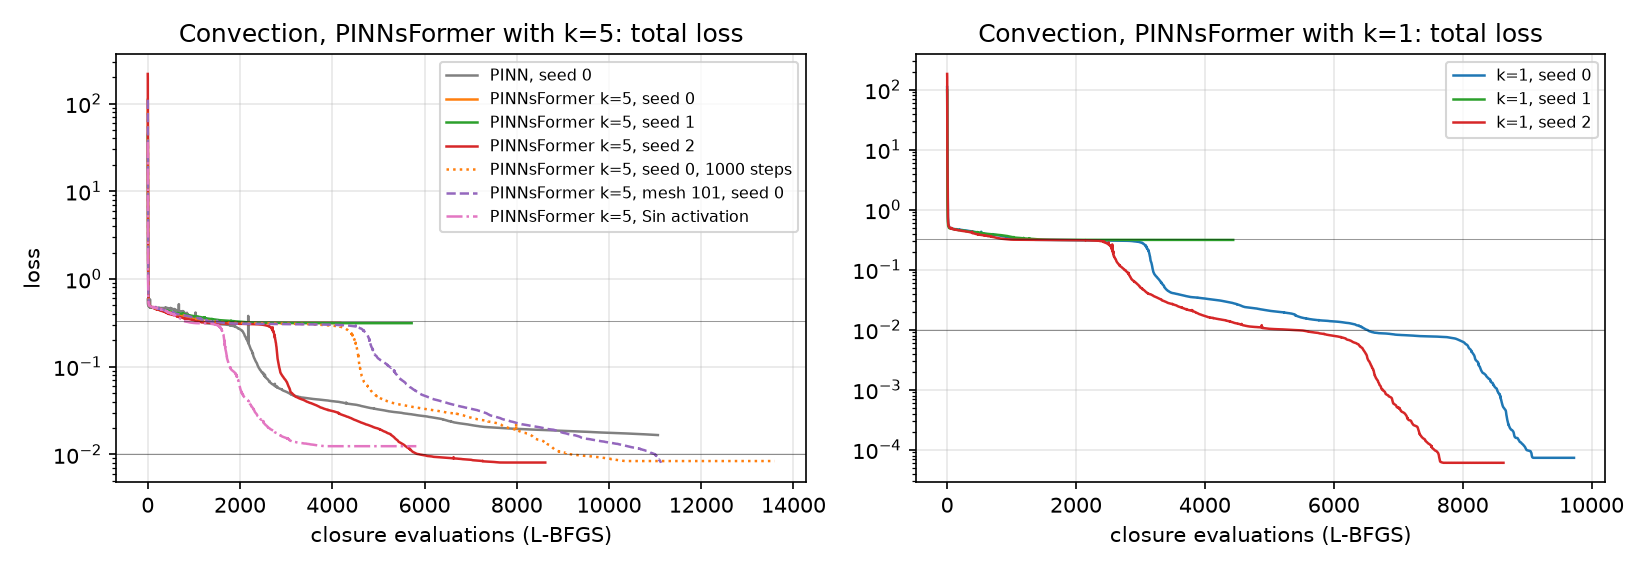
\includegraphics[width=0.9\textwidth]{fig_convection_loss.png}
\end{center}
\caption{Convection: training loss against L-BFGS closure evaluations. Left: the paper's $k=5$ configuration for three seeds, plus the 1000-step, mesh-101 and Sin-activation variants, with the PINN for reference. Right: $k=1$ for three seeds. The horizontal lines mark the constant plateau ($0.33$) and the PINN failure basin ($0.01$). No $k=5$ run reaches the true solution; two $k=1$ runs do.}
\label{fig:convloss}
\end{figure}

\begin{figure}[ht]
\begin{center}
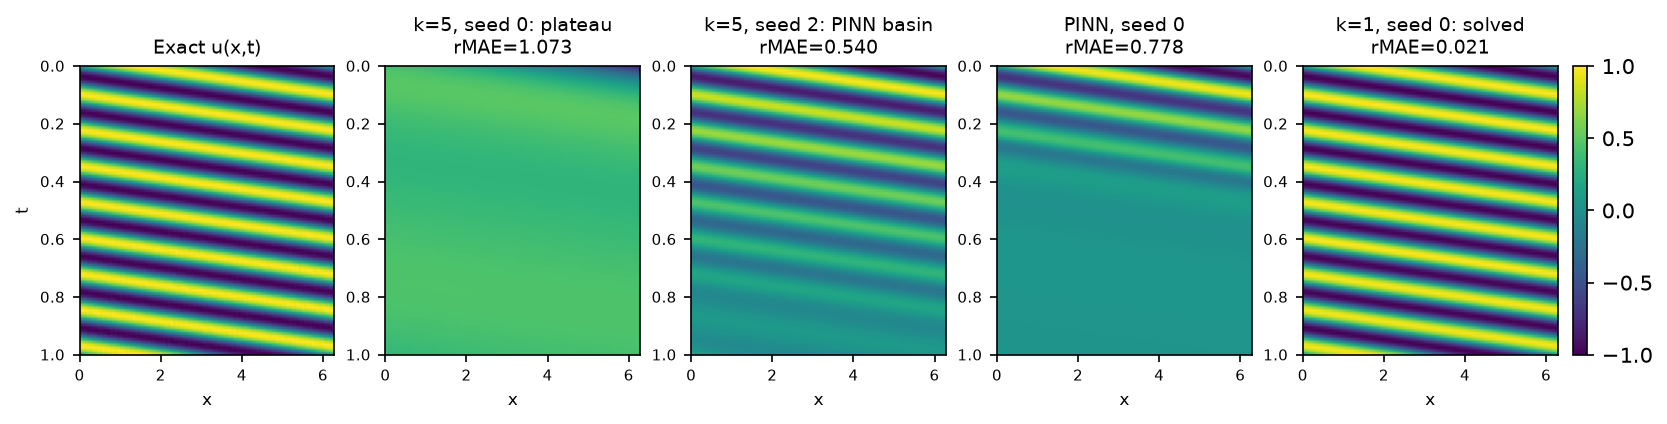
\includegraphics[width=0.92\textwidth]{fig_conv_pred_row.png}
\end{center}
\caption{Convection: exact solution and predictions of PINNsFormer $k=5$ seed 0 (constant plateau), $k=5$ seed 2 and the PINN (the classic failure mode: accurate near $t=0$, then decaying), and PINNsFormer $k=1$ seed 0 (solved).}
\label{fig:convpred}
\end{figure}

The seed column matters for both equations. The plain PINN on 1D-reaction solves the problem on one seed out of three (rMAE $0.064$) and fails on the other two, so the published single-seed row of $0.982$ is one draw from a bimodal distribution. Conversely PINNsFormer on convection ranges from $0.54$ to $1.07$. Neither comparison in Table~1 of the paper can be settled from single runs.

As a check independent of our training runs, we evaluated the shipped PINNsFormer checkpoints on the test mesh: convection gives rMAE $0.0229$ / rRMSE $0.0268$, matching the published $0.023$ / $0.027$; 1D-reaction gives $0.0231$ / $0.0449$ against $0.015$ / $0.030$, a gap the checkpoint README anticipates. Both are far from the failure regime, so the checkpoints support Claim~1 independently of whether training reproduces.

\subsubsection{Is Wavelet necessary? (Claim 2)}
\begin{table}[ht]
\caption{Activation ablation inside PINNsFormer (seed 0, 500 steps), compared with Table~6 of the paper.}
\label{tab:act}
\begin{center}
\small
\begin{tabular}{l cc cc cc cc}
\toprule
 & \multicolumn{4}{c}{Convection} & \multicolumn{4}{c}{1D-reaction} \\
 & \multicolumn{2}{c}{rMAE} & \multicolumn{2}{c}{rRMSE} & \multicolumn{2}{c}{rMAE} & \multicolumn{2}{c}{rRMSE} \\
Activation & Paper & Ours & Paper & Ours & Paper & Ours & Paper & Ours \\
\midrule
ReLU    & 1.001 & 1.001 & 1.001 & 1.002 & 0.994 & 0.992 & 0.996 & 0.995 \\
Sin     & 1.074 & 0.701 & 1.141 & 0.775 & 0.017 & 0.013 & 0.032 & 0.025 \\
Wavelet & 0.023 & 1.073 & 0.027 & 1.140 & 0.015 & 0.013 & 0.030 & 0.024 \\
\bottomrule
\end{tabular}
\end{center}
\end{table}

Table~\ref{tab:act} reproduces the paper's ablation for ReLU and Sin. ReLU fails on both equations, matching the published rows to three digits, as expected since the residual needs network derivatives and ReLU's is piecewise constant. Sin matches Wavelet on 1D-reaction ($0.013$ against $0.013$; the paper reports $0.017$ against $0.015$) and on convection ends in the PINN failure basin ($0.701$), better than the paper's Sin row ($1.074$) and than any of our five Wavelet runs. Claim~2 is thus supported against ReLU but not against Sin, which is unsurprising once the activation is written out: with both weights initialised to one, $\texttt{Wavelet}(x)=\sin x+\cos x=\sqrt{2}\sin(x+\pi/4)$, so it is a sine whose two learnable weights adjust amplitude and phase. Proposition~1 of the paper (universal approximation) holds equally for Sin, Tanh and ReLU and cannot explain differences between them.

The repository contains no code for this ablation; we replace all twelve Wavelet modules including the two in the output MLP, which is the most literal reading of the paper's description, and note that keeping Wavelet in the output MLP is an alternative we did not test.

\subsubsection{Overhead (Claim 4)}
With the paper's meshes, PINNsFormer on convection costs $1.2$--$2.7$\,s per step and $2262$\,MiB against $1.06$\,s and $822$\,MiB for the PINN, i.e.\ $1$--$2.5\times$ the time and $2.75\times$ the memory (paper: $2.9\times$ and $2.15\times$). The ratio is not architectural, since the models see different numbers of points: on matched $51\times51$ meshes it is $3$--$6\times$ and $4.2\times$, and on matched $101\times101$ meshes $11\times$ and $9\times$ ($11.4$\,s per step, $7646$\,MiB; Table~\ref{tab:allruns}). The paper does not say which mesh its Table~5 refers to.

\subsubsection{1D-wave (Claim 3)}
We ran the first two rows of the paper's Table~2 (without NTK) for 1000 steps. Our PINN reaches rMAE $0.099$ / rRMSE $0.114$, three times better than the paper's PINN ($0.326$ / $0.335$), while our PINNsFormer reaches $0.374$ / $0.378$, worse than the paper's $0.270$ / $0.283$. The ordering of the two models is therefore reversed. The NTK variants were not run, so we make no statement about the combined PINNsFormer+NTK result.

\subsection{Results beyond original paper}
\label{sec:beyond}
\begin{table}[ht]
\caption{Additional experiments (seed 0, 500 steps, rMAE / rRMSE). The first row repeats the paper's configuration for reference.}
\label{tab:beyond}
\begin{center}
\small
\begin{tabular}{l l cc cc}
\toprule
 & & \multicolumn{2}{c}{Convection} & \multicolumn{2}{c}{1D-reaction} \\
Question & Configuration & rMAE & rRMSE & rMAE & rRMSE \\
\midrule
reference & PINNsFormer, $k=5$, mesh 51 & 1.073 & 1.140 & 0.013 & 0.024 \\
activation alone? & PINN with Wavelet, mesh 101 & 1.262 & 1.392 & 0.984 & 0.989 \\
sequence needed? & PINNsFormer, $k=1$, mesh 51 & \textbf{0.021} & \textbf{0.025} & 0.977 & 0.977 \\
more points? & PINNsFormer, $k=5$, mesh 101 & 0.528 & 0.589 & 0.975 & 0.973 \\
fewer points? & PINN, mesh 51 & 0.736 & 0.805 & 0.980 & 0.981 \\
\bottomrule
\end{tabular}
\end{center}
\end{table}

\subsubsection{Is it the activation? PINN + Wavelet}
Replacing every Tanh in the PINN by the Wavelet activation does not help: the model fails on both equations (rMAE $1.26$ and $0.98$), on convection even more badly than the Tanh PINN. The activation alone therefore does not explain PINNsFormer's result on 1D-reaction. The paper's ablation (Table~6) only tests the converse, removing Wavelet from PINNsFormer.

\subsubsection{Is it the pseudo-sequence? PINNsFormer with $k=1$}
With $k=1$ the input is a single point, attention reduces to a per-point transformation, and no temporal dependency can be modelled. This configuration solves convection on two of three seeds (rMAE $0.021$ and $0.023$, matching the paper's headline number of $0.023$), while the paper's own $k=5$ configuration solved it on none of five runs. The failing $k=1$ seed is seed 1, which also fails with $k=5$: it stays on the constant plateau in both cases, so the plateau escape is decided by the initialisation rather than by the sequence length. On 1D-reaction the outcome is reversed: $k=1$ fails ($0.977$) and $k=5$ succeeds on all three seeds. The pseudo-sequence is thus not what makes convection solvable, and the paper's explanation in terms of temporal dependencies is not supported by this equation; on 1D-reaction it remains a possible explanation.

\subsubsection{Matched training meshes}
Giving PINNsFormer the baselines' $101\times101$ mesh makes it worse on both equations ($0.53$ and $0.98$) at $4$--$10\times$ the compute; giving the PINN the $51\times51$ mesh changes little ($0.74$ and $0.98$). On convection the mesh-101 run leaves the plateau only after $4700$ evaluations and is still descending at the budget's end (Figure~\ref{fig:convloss}, dashed), so it is budget-limited. Either way the smaller mesh is not a handicap PINNsFormer overcomes, as the paper suggests, but part of the configuration under which it converges in 500 steps.

\section{Discussion}
Our judgement per claim is as follows.
\begin{itemize}
    \item \textbf{Claim 1} is supported for 1D-reaction and not supported for convection. The baselines fail as published on both, but PINNsFormer's convection result could only be confirmed through the authors' checkpoint, not through training with their code and settings on our hardware.
    \item \textbf{Claim 2} is supported against ReLU and not against Sin: a plain sine activation performs as well as Wavelet on 1D-reaction and better in our convection runs, consistent with Wavelet being a phase-shifted sine with a learnable amplitude.
    \item \textbf{Claim 3} is not supported in the part we tested: the plain PINN beat PINNsFormer on 1D-wave and was much better than the paper's own PINN row.
    \item \textbf{Claim 4} holds in order of magnitude on the paper's meshes but understates the cost on equal meshes by a factor of four to five.
    \item \textbf{Claim 5}, the paper's explanation, is contradicted on convection: without any pseudo-sequence ($k=1$) the method solves the equation on two seeds of three, with the paper's $k=5$ on none of five runs, and doubling the iteration budget does not change this. On 1D-reaction the sequence does appear to matter, so the explanation may hold for some equations but is not general.
\end{itemize}
The strongest finding is the sensitivity itself: three seeds of one configuration span rMAE $0.54$--$1.07$ on convection, and a baseline the paper reports as failing solves 1D-reaction on one seed. Both point to the optimiser, L-BFGS on a non-convex loss, as the dominant factor, and suggest that the paper's loss-landscape argument (a single Lipschitz estimate on one trained model) is too weak to carry the claim. Our study has the mirror limitation: three seeds, two equations and 500 steps are enough to show fragility, not to characterise it.

\subsection{What was easy}
The repository has one notebook per experiment, short model files, a mesh utility and pretrained checkpoints; the problems fit in a few GPU hours on free Colab; and because every loss term is written out in the notebooks, checking them against Equation~6 of the paper and factoring them into one script was straightforward.

\subsection{What was difficult}
The difficulties were about matching the paper to the code rather than about running it. We found the following undocumented discrepancies: (i) the paper states 1000 training iterations, the convection and 1D-reaction notebooks run 500 L-BFGS steps (1D-wave: 1000), and each ``iteration'' is one L-BFGS step with up to 20 inner evaluations; (ii) the wave coefficient is $\beta=3$ in the text but $4$ in the code and in the paper's own analytic solution; (iii) the ``hidden size'' of 512 in Table~4 is the output MLP, while the feed-forward blocks inside the encoder and decoder are hard-coded to 256, and the stated 454k parameters are only obtained with that setting; (iv) QRes has 4 blocks of width 256 in the 1D-reaction notebook (matching Table~4) but 2 blocks of width 512 in the convection notebook; (v) $\Delta t$ is $10^{-4}$ in every notebook except the 1D-wave NTK notebook ($10^{-3}$), and the paper lists both without saying which is which; (vi) the caption of Figure~8 says 1D-reaction but shows 1D-wave; (vii) baselines and PINNsFormer are trained on different meshes and results are single-seed; (viii) the environment file pins PyTorch 2.0.1 and CUDA 11.6, and the checkpoint README warns that results may not match across versions. Practically, free Colab assigned a different GPU (L4) to our second session; we logged the device per run and made the sweep resumable so that a disconnect only costs the run in progress.

\subsection{Communication with original authors}
We did not contact the authors. The questions we would have asked are recorded above: whether the published numbers were obtained with 500 or 1000 L-BFGS steps, which QRes configuration Table~1 uses, and whether the Table~6 ablation also replaced the activations of the output MLP. All three could be settled by the authors in a few lines and would remove most of the ambiguity in this study.

\section{Conclusion}
Using the authors' code, we reproduced the 1D-reaction result of PINNsFormer and the failure of the MLP baselines there, but not the convection result: the paper's configuration fell into a constant plateau or the classic PINN failure mode on every run, while the authors' checkpoint solves the problem, and on 1D-wave the plain PINN won. Controlled experiments the paper lacks point to optimisation rather than architecture: seeds change the outcome for baselines and PINNsFormer alike, removing the pseudo-sequence made convection easier, a plain sine matched the Wavelet activation, and a larger mesh did not help. The empirical claim thus holds on one of its two equations, and the explanation in terms of temporal dependencies is not supported. A convincing follow-up would compare all models over many seeds on equal meshes with a fixed evaluation budget, separating the contributions of the sine activation, the encoder--decoder and the reduced mesh.

\section*{Member contributions}
Single-student project: literature study, code analysis, all experiments, report and presentation by the author.

%%%%

\bibliography{main}
\bibliographystyle{tmlr}

\appendix
\section{All runs}
Table~\ref{tab:allruns} lists every training run of this study. Runs are identified by model, training mesh (points per axis), number of L-BFGS steps and seed. The per-run outputs (prediction on the test mesh, loss per closure evaluation, figure and configuration) are included in the submitted code archive under \texttt{results/}.

\begin{table}[ht]
\caption{All 34 training runs. Time is wall-clock training time in minutes; memory is peak GPU memory in MiB. Runs 28--34 (1000-step run, $k=1$ seeds 1--2, Sin/ReLU) ran on an L4, all others on a T4.}
\label{tab:allruns}
\begin{center}
\scriptsize
\begin{tabular}{l r r r r r r r}
\toprule
Model & Mesh & Steps & Seed & Loss & rMAE & rRMSE & Time / Mem \\
\midrule
\multicolumn{8}{l}{\textit{Convection}} \\
FLS & 101 & 500 & 0 & 1.10e-02 & 0.662 & 0.743 & 8.3 / 847 \\
PINN & 51 & 500 & 0 & 1.36e-02 & 0.736 & 0.805 & 3.8 / 544 \\
PINN & 101 & 500 & 0 & 1.66e-02 & 0.778 & 0.841 & 8.8 / 822 \\
PINN & 101 & 500 & 1 & 2.46e-02 & 0.857 & 0.904 & 5.0 / 826 \\
PINN & 101 & 500 & 2 & 1.58e-02 & 0.766 & 0.830 & 9.0 / 822 \\
PINN+Wavelet & 101 & 500 & 0 & 4.70e-01 & 1.262 & 1.392 & 3.8 / 1313 \\
PINNsFormer, $k=1$ & 51 & 500 & 0 & 7.32e-05 & 0.021 & 0.025 & 11.2 / 772 \\
PINNsFormer, $k=1$ & 51 & 500 & 1 & 3.13e-01 & 1.066 & 1.128 & 4.4 / 772 \\
PINNsFormer, $k=1$ & 51 & 500 & 2 & 6.05e-05 & 0.023 & 0.026 & 9.6 / 772 \\
PINNsFormer, $k=5$, ReLU & 51 & 500 & 0 & 5.61e-01 & 1.001 & 1.002 & 3.9 / 586 \\
PINNsFormer, $k=5$, Sin & 51 & 500 & 0 & 1.24e-02 & 0.701 & 0.775 & 5.9 / 1357 \\
PINNsFormer, $k=5$ & 51 & 500 & 0 & 3.15e-01 & 1.073 & 1.140 & 10.3 / 2262 \\
PINNsFormer, $k=5$ & 51 & 500 & 1 & 3.13e-01 & 1.066 & 1.129 & 14.4 / 2262 \\
PINNsFormer, $k=5$ & 51 & 500 & 2 & 8.07e-03 & 0.540 & 0.619 & 22.1 / 2262 \\
PINNsFormer, $k=5$ & 51 & 1000 & 0 & 8.39e-03 & 0.548 & 0.626 & 25.3 / 2264 \\
PINNsFormer, $k=5$ & 101 & 500 & 0 & 8.01e-03 & 0.528 & 0.589 & 95.3 / 7646 \\
QRes & 101 & 500 & 0 & 4.89e-02 & 0.947 & 0.993 & 5.1 / 836 \\
QRes (512$\times$2) & 101 & 500 & 0 & 1.60e-01 & 1.029 & 1.086 & 3.2 / 988 \\
\midrule
\multicolumn{8}{l}{\textit{1D-reaction}} \\
FLS & 101 & 500 & 0 & 1.99e-01 & 0.985 & 0.984 & 2.4 / 727 \\
PINN & 51 & 500 & 0 & 1.98e-01 & 0.980 & 0.981 & 0.7 / 519 \\
PINN & 101 & 500 & 0 & 1.99e-01 & 0.979 & 0.978 & 2.2 / 726 \\
PINN & 101 & 500 & 1 & 1.99e-01 & 0.979 & 0.977 & 1.7 / 726 \\
PINN & 101 & 500 & 2 & 9.97e-05 & 0.064 & 0.104 & 3.5 / 726 \\
PINN+Wavelet & 101 & 500 & 0 & 2.04e-01 & 0.984 & 0.989 & 2.7 / 1070 \\
PINNsFormer, $k=1$ & 51 & 500 & 0 & 1.98e-01 & 0.977 & 0.977 & 2.3 / 648 \\
PINNsFormer, $k=5$, ReLU & 51 & 500 & 0 & 2.07e-01 & 0.992 & 0.995 & 3.1 / 537 \\
PINNsFormer, $k=5$, Sin & 51 & 500 & 0 & 5.49e-06 & 0.013 & 0.025 & 3.2 / 1039 \\
PINNsFormer, $k=5$ & 51 & 500 & 0 & 4.44e-06 & 0.013 & 0.024 & 5.2 / 1627 \\
PINNsFormer, $k=5$ & 51 & 500 & 1 & 4.25e-06 & 0.018 & 0.036 & 3.1 / 1627 \\
PINNsFormer, $k=5$ & 51 & 500 & 2 & 5.08e-06 & 0.018 & 0.036 & 3.3 / 1627 \\
PINNsFormer, $k=5$ & 101 & 500 & 0 & 1.99e-01 & 0.975 & 0.973 & 14.8 / 5178 \\
QRes & 101 & 500 & 0 & 1.99e-01 & 0.986 & 0.986 & 2.0 / 686 \\
\midrule
\multicolumn{8}{l}{\textit{1D-wave}} \\
PINN & 101 & 1000 & 0 & 3.36e-03 & 0.099 & 0.114 & 33.2 / 1468 \\
PINNsFormer, $k=5$ & 51 & 1000 & 0 & 2.36e-02 & 0.374 & 0.378 & 82.5 / 5063 \\
\bottomrule
\end{tabular}
\end{center}
\end{table}


\end{document}
